\documentclass{standalone}
\usepackage{tikz}
\usetikzlibrary{patterns, positioning}

\begin{document}
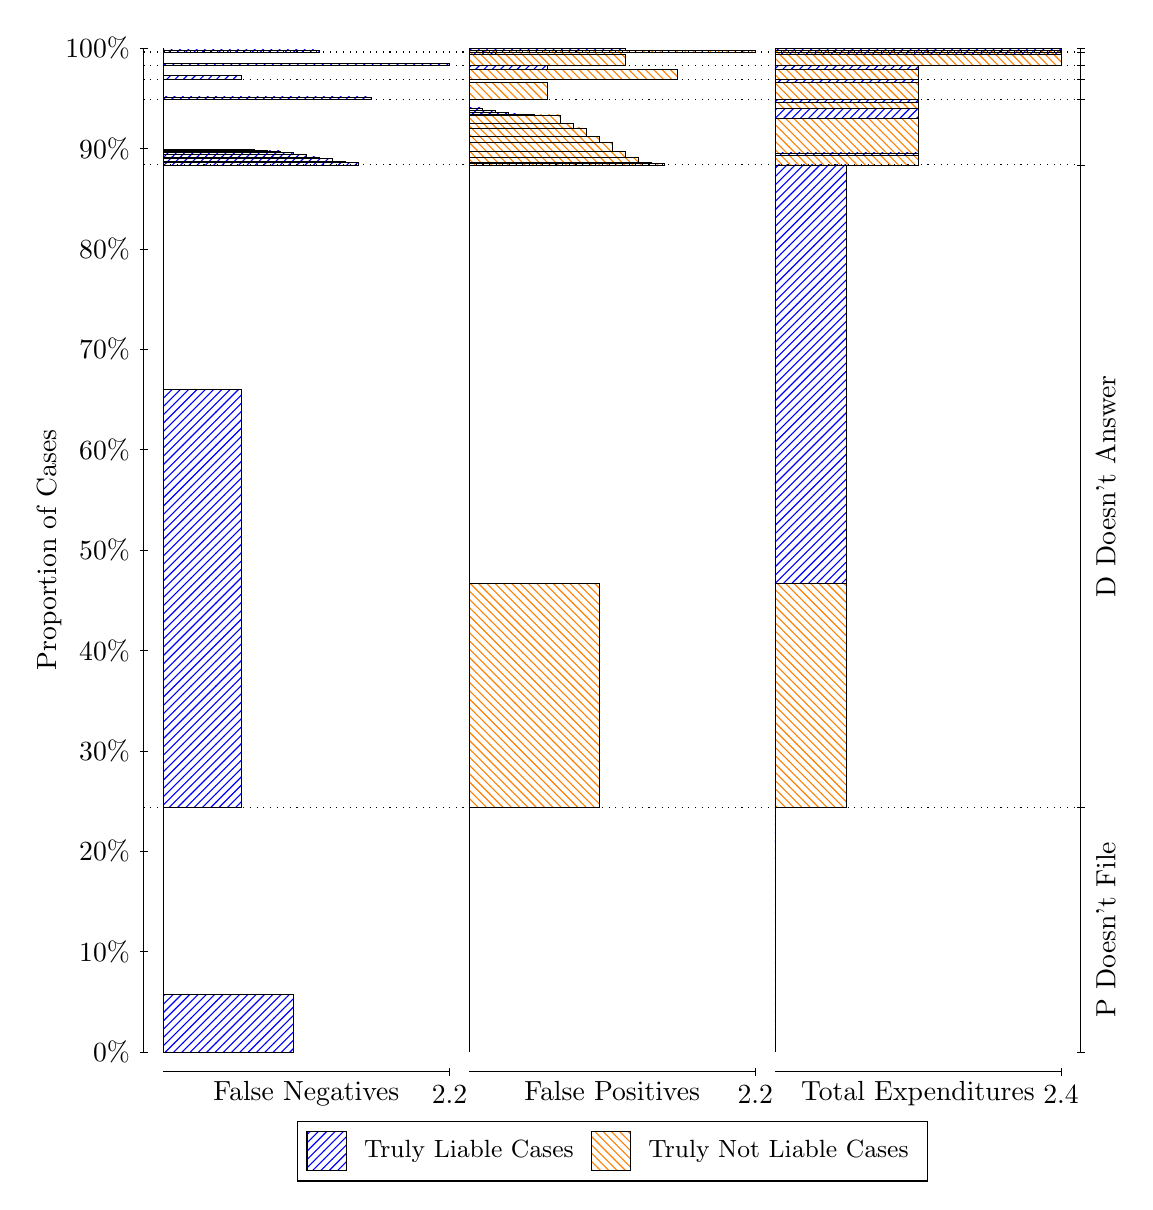
\begin{tikzpicture}
\draw[black, very thin] (1.5,1.75) -- (1.5,14.5);
\node[rotate=90, anchor=center] at (0.3, 8.125) {Proportion of Cases};
\draw[black, very thin] (1.45,1.75) -- (1.55,1.75);
\node[anchor=east] at (1.45, 1.75) {0\%};
\draw[black, very thin] (1.45,3.025) -- (1.55,3.025);
\node[anchor=east] at (1.45, 3.025) {10\%};
\draw[black, very thin] (1.45,4.3) -- (1.55,4.3);
\node[anchor=east] at (1.45, 4.3) {20\%};
\draw[black, very thin] (1.45,5.575) -- (1.55,5.575);
\node[anchor=east] at (1.45, 5.575) {30\%};
\draw[black, very thin] (1.45,6.85) -- (1.55,6.85);
\node[anchor=east] at (1.45, 6.85) {40\%};
\draw[black, very thin] (1.45,8.125) -- (1.55,8.125);
\node[anchor=east] at (1.45, 8.125) {50\%};
\draw[black, very thin] (1.45,9.4) -- (1.55,9.4);
\node[anchor=east] at (1.45, 9.4) {60\%};
\draw[black, very thin] (1.45,10.675) -- (1.55,10.675);
\node[anchor=east] at (1.45, 10.675) {70\%};
\draw[black, very thin] (1.45,11.95) -- (1.55,11.95);
\node[anchor=east] at (1.45, 11.95) {80\%};
\draw[black, very thin] (1.45,13.225) -- (1.55,13.225);
\node[anchor=east] at (1.45, 13.225) {90\%};
\draw[black, very thin] (1.45,14.5) -- (1.55,14.5);
\node[anchor=east] at (1.45, 14.5) {100\%};

\draw[black, very thin] (13.4,1.75) -- (13.4,14.5);
\draw[black, very thin] (13.35,1.75) -- (13.45,1.75);
\node[anchor=west] at (13.35, 1.75) {};
\draw[black, very thin] (13.35,4.8554) -- (13.45,4.8554);
\node[anchor=west] at (13.35, 4.8554) {};
\draw[black, very thin] (13.35,13.016) -- (13.45,13.016);
\node[anchor=west] at (13.35, 13.016) {};
\draw[black, very thin] (13.35,13.843) -- (13.45,13.843);
\node[anchor=west] at (13.35, 13.843) {};
\draw[black, very thin] (13.35,14.101) -- (13.45,14.101);
\node[anchor=west] at (13.35, 14.101) {};
\draw[black, very thin] (13.35,14.277) -- (13.45,14.277);
\node[anchor=west] at (13.35, 14.277) {};
\draw[black, very thin] (13.35,14.45) -- (13.45,14.45);
\node[anchor=west] at (13.35, 14.45) {};
\draw[black, very thin] (13.35,14.5) -- (13.45,14.5);
\node[anchor=west] at (13.35, 14.5) {};

\draw[black, very thin, pattern color=blue, pattern=north east lines] (1.75,1.75) rectangle (3.4015,2.4778);
\draw[black, very thin, pattern color=orange, pattern=north west lines] (1.75,2.4778) rectangle (1.75,4.8554);
\draw[black, very thin, pattern color=blue, pattern=north east lines] (1.75,4.8554) rectangle (2.7409,10.169);
\draw[black, very thin, pattern color=orange, pattern=north west lines] (1.75,10.169) rectangle (1.75,13.016);
\draw[black, very thin, pattern color=blue, pattern=north east lines] (1.75,13.016) rectangle (4.2273,13.043);
\draw[black, very thin, pattern color=blue, pattern=north east lines] (1.75,13.043) rectangle (4.0621,13.065);
\draw[black, very thin, pattern color=blue, pattern=north east lines] (1.75,13.065) rectangle (3.897,13.095);
\draw[black, very thin, pattern color=blue, pattern=north east lines] (1.75,13.095) rectangle (3.7318,13.117);
\draw[black, very thin, pattern color=blue, pattern=north east lines] (1.75,13.117) rectangle (3.5667,13.152);
\draw[black, very thin, pattern color=blue, pattern=north east lines] (1.75,13.152) rectangle (3.4015,13.174);
\draw[black, very thin, pattern color=blue, pattern=north east lines] (1.75,13.174) rectangle (3.2364,13.195);
\draw[black, very thin, pattern color=blue, pattern=north east lines] (1.75,13.195) rectangle (3.0712,13.204);
\draw[black, very thin, pattern color=blue, pattern=north east lines] (1.75,13.204) rectangle (2.9061,13.208);
\draw[black, very thin, pattern color=orange, pattern=north west lines] (1.75,13.208) rectangle (1.75,13.843);
\draw[black, very thin, pattern color=blue, pattern=north east lines] (1.75,13.843) rectangle (4.3924,13.88);
\draw[black, very thin, pattern color=orange, pattern=north west lines] (1.75,13.88) rectangle (1.75,14.101);
\draw[black, very thin, pattern color=blue, pattern=north east lines] (1.75,14.101) rectangle (2.7409,14.155);
\draw[black, very thin, pattern color=orange, pattern=north west lines] (1.75,14.155) rectangle (1.75,14.277);
\draw[black, very thin, pattern color=blue, pattern=north east lines] (1.75,14.277) rectangle (5.3833,14.302);
\draw[black, very thin, pattern color=orange, pattern=north west lines] (1.75,14.302) rectangle (1.75,14.45);
\draw[black, very thin, pattern color=blue, pattern=north east lines] (1.75,14.45) rectangle (3.7318,14.476);
\draw[black, very thin, pattern color=orange, pattern=north west lines] (1.75,14.476) rectangle (1.75,14.5);
\draw[black, very thin, pattern color=orange, pattern=north west lines] (5.6333,1.75) rectangle (5.6333,4.1276);
\draw[black, very thin, pattern color=blue, pattern=north east lines] (5.6333,4.1276) rectangle (5.6333,4.8554);
\draw[black, very thin, pattern color=orange, pattern=north west lines] (5.6333,4.8554) rectangle (7.2848,7.7023);
\draw[black, very thin, pattern color=blue, pattern=north east lines] (5.6333,7.7023) rectangle (5.6333,13.016);
\draw[black, very thin, pattern color=orange, pattern=north west lines] (5.6333,13.016) rectangle (8.1106,13.032);
\draw[black, very thin, pattern color=orange, pattern=north west lines] (5.6333,13.032) rectangle (7.9455,13.05);
\draw[black, very thin, pattern color=orange, pattern=north west lines] (5.6333,13.05) rectangle (7.7803,13.107);
\draw[black, very thin, pattern color=orange, pattern=north west lines] (5.6333,13.107) rectangle (7.6152,13.187);
\draw[black, very thin, pattern color=orange, pattern=north west lines] (5.6333,13.187) rectangle (7.45,13.304);
\draw[black, very thin, pattern color=orange, pattern=north west lines] (5.6333,13.304) rectangle (7.2848,13.381);
\draw[black, very thin, pattern color=orange, pattern=north west lines] (5.6333,13.381) rectangle (7.1197,13.485);
\draw[black, very thin, pattern color=orange, pattern=north west lines] (5.6333,13.485) rectangle (6.9545,13.544);
\draw[black, very thin, pattern color=orange, pattern=north west lines] (5.6333,13.544) rectangle (6.7894,13.65);
\draw[black, very thin, pattern color=blue, pattern=north east lines] (5.6333,13.65) rectangle (6.4591,13.654);
\draw[black, very thin, pattern color=blue, pattern=north east lines] (5.6333,13.654) rectangle (6.2939,13.663);
\draw[black, very thin, pattern color=blue, pattern=north east lines] (5.6333,13.663) rectangle (6.1288,13.684);
\draw[black, very thin, pattern color=blue, pattern=north east lines] (5.6333,13.684) rectangle (5.9636,13.707);
\draw[black, very thin, pattern color=blue, pattern=north east lines] (5.6333,13.707) rectangle (5.7985,13.741);
\draw[black, very thin, pattern color=blue, pattern=north east lines] (5.6333,13.741) rectangle (5.6333,13.843);
\draw[black, very thin, pattern color=orange, pattern=north west lines] (5.6333,13.843) rectangle (6.6242,14.064);
\draw[black, very thin, pattern color=blue, pattern=north east lines] (5.6333,14.064) rectangle (5.6333,14.101);
\draw[black, very thin, pattern color=orange, pattern=north west lines] (5.6333,14.101) rectangle (8.2758,14.224);
\draw[black, very thin, pattern color=blue, pattern=north east lines] (5.6333,14.224) rectangle (6.6242,14.277);
\draw[black, very thin, pattern color=orange, pattern=north west lines] (5.6333,14.277) rectangle (7.6152,14.426);
\draw[black, very thin, pattern color=blue, pattern=north east lines] (5.6333,14.426) rectangle (5.9636,14.45);
\draw[black, very thin, pattern color=orange, pattern=north west lines] (5.6333,14.45) rectangle (9.2667,14.474);
\draw[black, very thin, pattern color=blue, pattern=north east lines] (5.6333,14.474) rectangle (7.6152,14.5);
\draw[black, very thin, pattern color=orange, pattern=north west lines] (9.5167,1.75) rectangle (9.5167,4.1276);
\draw[black, very thin, pattern color=blue, pattern=north east lines] (9.5167,4.1276) rectangle (9.5167,4.8554);
\draw[black, very thin, pattern color=orange, pattern=north west lines] (9.5167,4.8554) rectangle (10.425,7.7023);
\draw[black, very thin, pattern color=blue, pattern=north east lines] (9.5167,7.7023) rectangle (10.425,13.016);
\draw[black, very thin, pattern color=orange, pattern=north west lines] (9.5167,13.016) rectangle (11.333,13.132);
\draw[black, very thin, pattern color=blue, pattern=north east lines] (9.5167,13.132) rectangle (11.333,13.167);
\draw[black, very thin, pattern color=orange, pattern=north west lines] (9.5167,13.167) rectangle (11.333,13.61);
\draw[black, very thin, pattern color=blue, pattern=north east lines] (9.5167,13.61) rectangle (11.333,13.738);
\draw[black, very thin, pattern color=orange, pattern=north west lines] (9.5167,13.738) rectangle (11.333,13.813);
\draw[black, very thin, pattern color=blue, pattern=north east lines] (9.5167,13.813) rectangle (11.333,13.843);
\draw[black, very thin, pattern color=orange, pattern=north west lines] (9.5167,13.843) rectangle (11.333,14.064);
\draw[black, very thin, pattern color=blue, pattern=north east lines] (9.5167,14.064) rectangle (11.333,14.101);
\draw[black, very thin, pattern color=orange, pattern=north west lines] (9.5167,14.101) rectangle (11.333,14.224);
\draw[black, very thin, pattern color=blue, pattern=north east lines] (9.5167,14.224) rectangle (11.333,14.277);
\draw[black, very thin, pattern color=orange, pattern=north west lines] (9.5167,14.277) rectangle (13.15,14.426);
\draw[black, very thin, pattern color=blue, pattern=north east lines] (9.5167,14.426) rectangle (13.15,14.45);
\draw[black, very thin, pattern color=orange, pattern=north west lines] (9.5167,14.45) rectangle (13.15,14.474);
\draw[black, very thin, pattern color=blue, pattern=north east lines] (9.5167,14.474) rectangle (13.15,14.5);
\draw[black, dotted] (1.5,4.8554) -- (13.4,4.8554);
\draw[black, dotted] (1.5,13.016) -- (13.4,13.016);
\draw[black, dotted] (1.5,13.843) -- (13.4,13.843);
\draw[black, dotted] (1.5,14.101) -- (13.4,14.101);
\draw[black, dotted] (1.5,14.277) -- (13.4,14.277);
\draw[black, dotted] (1.5,14.45) -- (13.4,14.45);
\draw[black, very thin] (1.75,1.5) -- (5.3833,1.5);
\node[anchor=north] at (3.5667, 1.5) {False Negatives};
\draw[black, very thin] (5.3833,1.45) -- (5.3833,1.55);
\node[anchor=north] at (5.3833, 1.45) {2.2};

\draw[black, very thin] (5.6333,1.5) -- (9.2667,1.5);
\node[anchor=north] at (7.45, 1.5) {False Positives};
\draw[black, very thin] (9.2667,1.45) -- (9.2667,1.55);
\node[anchor=north] at (9.2667, 1.45) {2.2};

\draw[black, very thin] (9.5167,1.5) -- (13.15,1.5);
\node[anchor=north] at (11.333, 1.5) {Total Expenditures};
\draw[black, very thin] (13.15,1.45) -- (13.15,1.55);
\node[anchor=north] at (13.15, 1.45) {2.4};

\node[black, centered, rotate=90] at (13.72, 3.3027) {P Doesn't File};
\node[black, centered, rotate=90] at (13.72, 8.9354) {D Doesn't Answer};






\draw (7.449999999999999,1.5) node[draw=none] (baseCoordinate) {};
\begin{scope}[align=center]
        \matrix[scale=0.5, draw=black, below=0.5cm of baseCoordinate, nodes={draw}, column sep=0.1cm]{
            \node[rectangle, draw, minimum width=0.5cm, minimum height=0.5cm, pattern=north east lines, pattern color=blue] {}; &
            \node[draw=none, font=\small] (B) {Truly Liable Cases}; &
            \node[rectangle, draw, minimum width=0.5cm, minimum height=0.5cm, pattern=north west lines, pattern color=orange] {}; &
            \node[draw=none, font=\small] (B) {Truly Not Liable Cases}; \\
            };
\end{scope}

\end{tikzpicture}
\end{document}